\section{Architektur}

Dieses Kapitel erläutert den Aufbau unserer Applikation.
Auf der Abbildung \ref{fig:overview} sind die Klassen und Interfaces der Applikation ersichtlich.
Wir verwenden das Pipe and Filter Pattern. Dies ermöglicht es die Applikation um weitere Filter einfach zu erweitern. 

\begin{figure}[ht]
	\begin{center}
		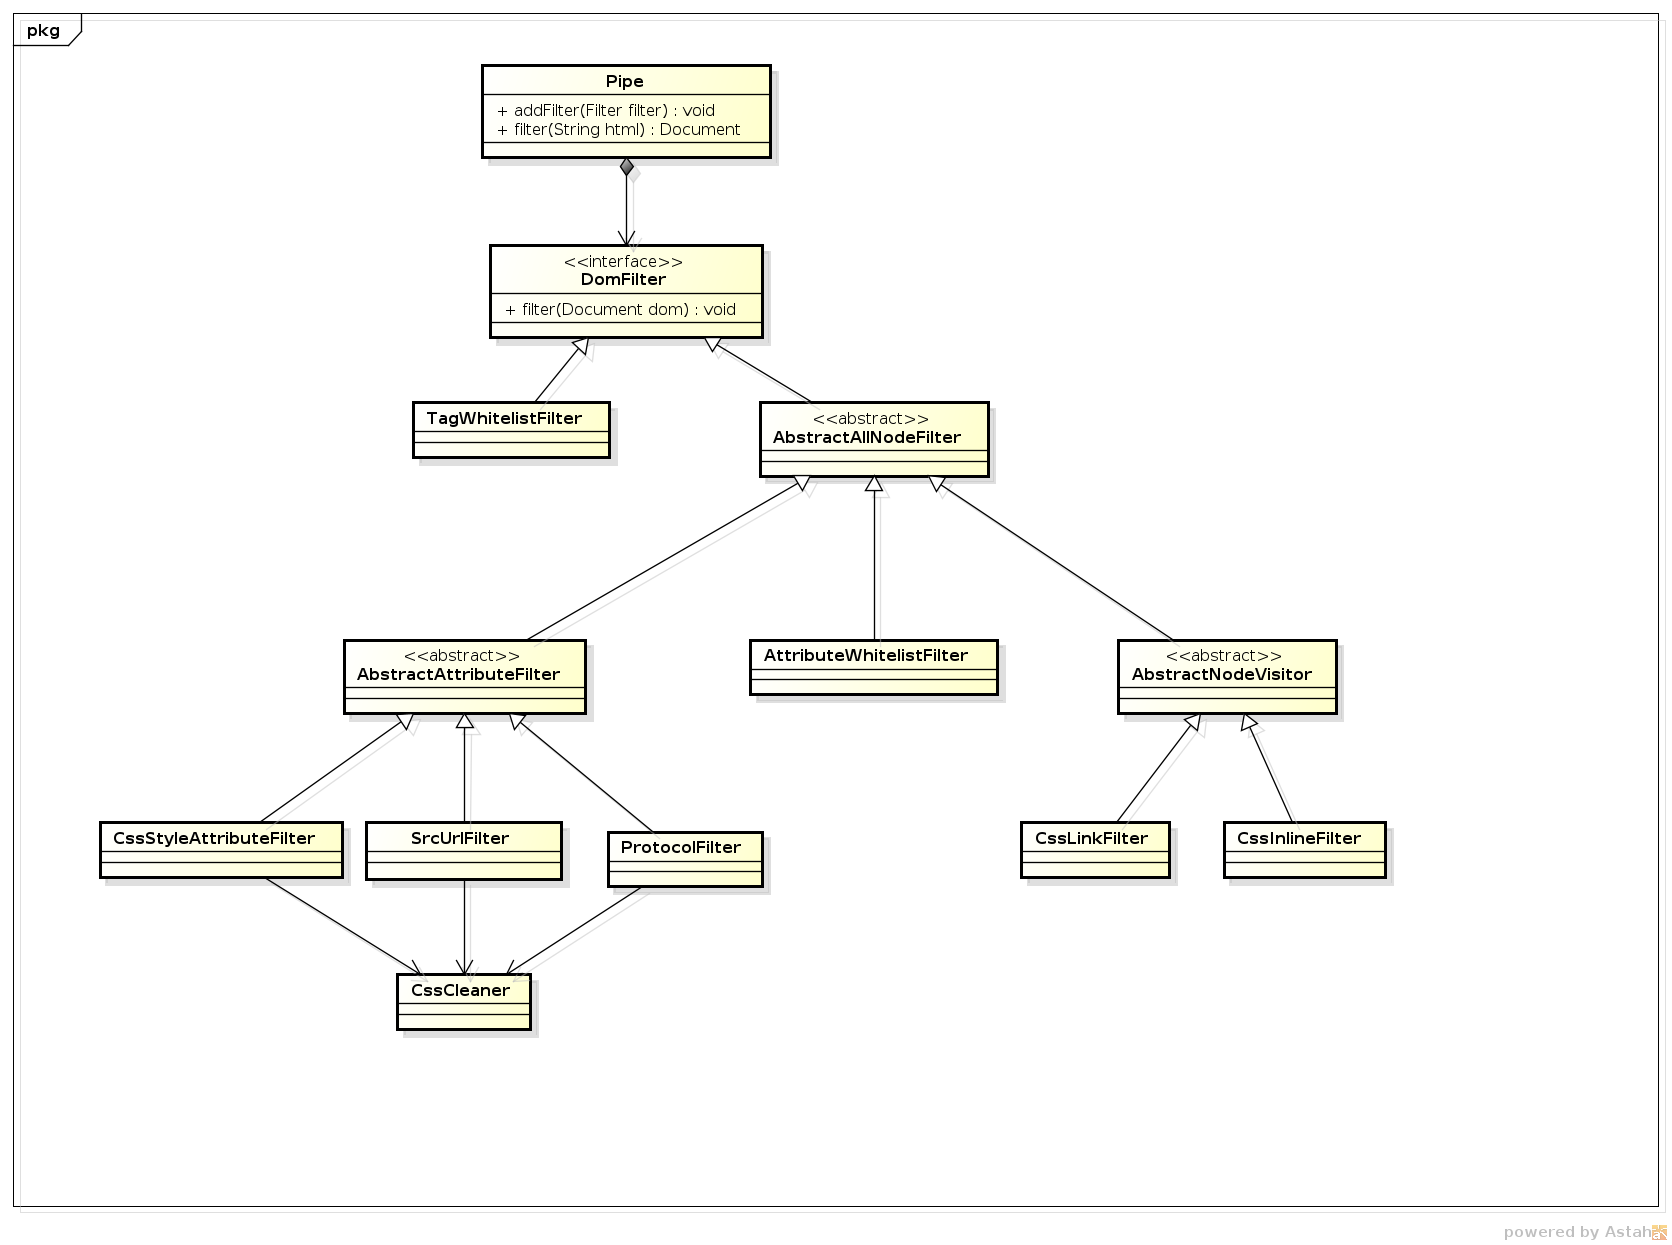
\includegraphics[width=1.0\textwidth]{./content/Class_Overview.png}
	\end{center}
	\caption{Übersicht über die Klassen und Interfaces}
	\label{fig:overview}
\end{figure}

\subsection{DOM Parser}

Eine sehr wichtige Komponente des Mail Filters ist der Parser, welcher das HTML in das Document
Object Model (DOM) verwandelt. Nebst dem Parsen ist er zusätzlich dafür verantwortlich, alle Character
Encodings korrekt zu interpretieren und in Java Unicode Character Strings zu verwandeln. Aus diesem 
Grund wurde viel Wert auf die Auswahl eines geeigneten Parsers gelegt. Wir entschieden uns am Schluss 
für den Parser \textit{jsoup}\cite{DOM:JSOUP}. Diese Opensource Bibliothek erfüllte alle unsere 
Anforderungen und ist zudem sehr gut dokumentiert. 

\subsection{Authentifizierung}

Um sicherzustellen, dass lediglich Benutzer mit Administrationsrechten die Applikation ausführen können,
haben wir die Authentifizierung mittels JAAS implementiert. Damit die Plattformunabhängigkeit 
gewährleistet bleibt, haben wir sowohl das Login für Windows, als auch für Unix basierte Systeme 
implementiert. Die JAAS-Konfiguration ist in Listing \ref{lst:jaas} ersichtlich. Dabei wird je
nach verwendetem System der entsprechende LoginContext geladen. Im Falle von Unix wird dabei auf eine
Gruppe 0 des angemeldeten Benutzer überprüft, im Falle von Windows auf die Well-known-group 
SID\cite{MS:SID} \textit{S-1-5-32-544}, welche die Gruppe der lokalen Administratoren identifiziert. 
\newline
\begin{lstlisting}[caption="JAAS konfiguration im File jaas\_security.conf", label={lst:jaas}]
Unix {
        com.sun.security.auth.module.UnixLoginModule required debug=false;
};

Windows {
        com.sun.security.auth.module.NTLoginModule required debug=false;
};
\end{lstlisting}

\newpage

\subsection{Verarbeitungsprozess}

Das Aktivitätsdiagramm Abbildung \ref{fig:process} beschreibt den Verarbeitungsprozess vom Starten der Applikation, bis zur Ausgabe des gesäuberten HTML Codes.

\begin{figure}[ht]
	\begin{center}
		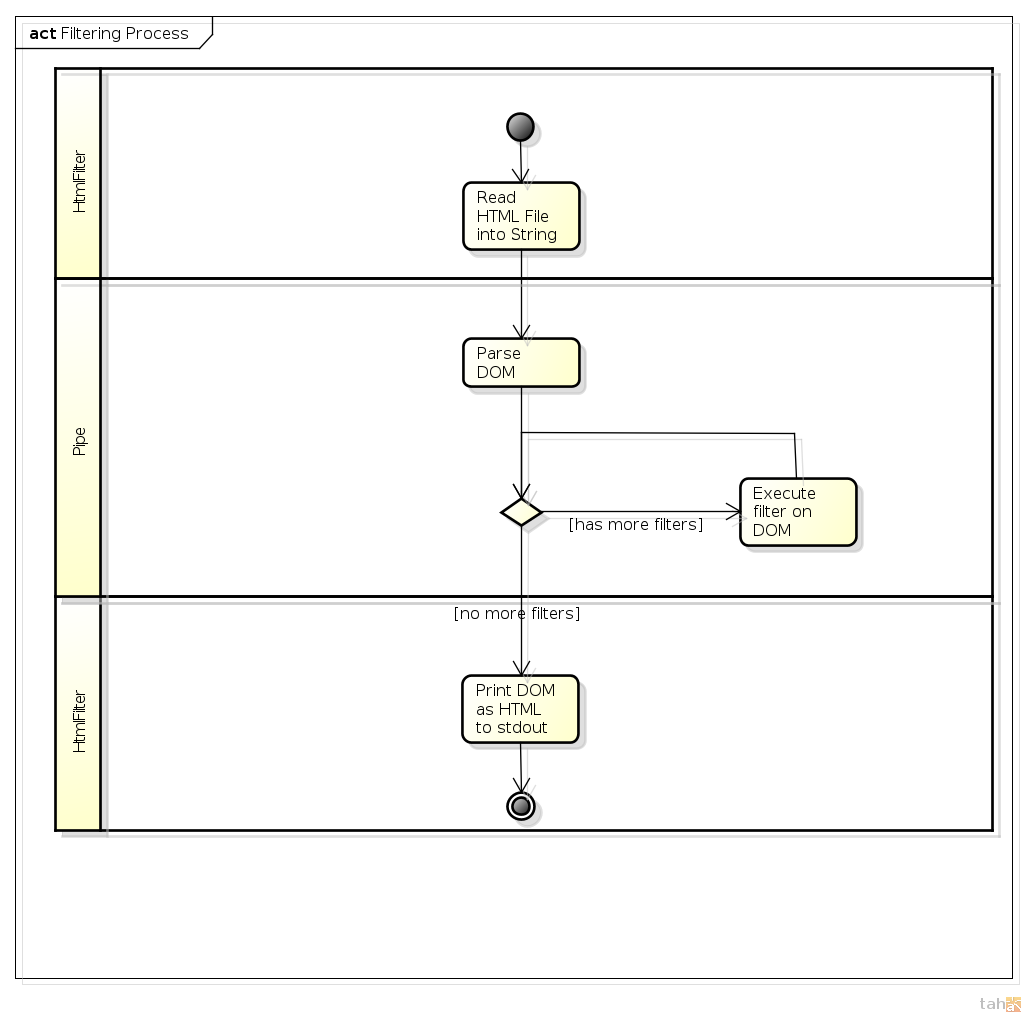
\includegraphics[width=1.0\textwidth]{./content/Filtering_Process_cut.png}
	\end{center}
	\caption{Verarbeitungsprozess}
	\label{fig:process}
\end{figure}

\subsection{Filter}

Dieser Abschnitt beschreibt die implementierten Filter. 
In der Tabelle \ref{tab:filter} sind die implementierten Filter aufgelistet. Die Filter operieren auf dem erstellten HTML-DOM.
Jeder Filter bekommt als Eingabe den HTML-Baum und gibt den gefilterten HTML-Baum zurück. 
Beim Filterprozess werden HTML und CSS Tags und Attribute entfernt, ersetzt und geändert.

\begin{table}[h!]
\begin{center}
\begin{tabular}{l p{10.5cm} }
\hline
\textbf{Filter} & \textbf{Beschreibung} \\ \hline \hline
TagWhitelistFilter & Dieser Filter entfernt alle HTML Tags welche nicht in der Whitelist enthalten sind. 
Beim Entfernen eines HTML Tags werden auch die zugehörigen HTML Child Nodes entfernt. \\ 

AttributeWhitelistFilter & Der Attribute Whitelist Filter entfernt alle HTML Attribute welche nicht in der Whitelist enthalten sind. \\

ProtocolFilter & Der Protocol Filter setzt bei den HTML Attributen href und src den Wert auf '', wenn das Protokoll nicht in der Whitelist vorhanden ist. \\

SrcUrlFilter & Dieser Filter entfernt den Query Parameter beim HTML src Attribut aus der URL. Dies verhindert z.B. folgende URLs http://www.test.com/test.php?somevariables=maliciouscode in img Tags. \\

CssCleaner & Dies ist kein Filter, wird aber von Css Filter Klassen verwendet. Der CssCleaner entfernt mit Hilfe von Regular Expressions -moz-binding, behavior, @import, expression und url Tags. \\

CssStyleAttributeFilter & Dieser Filter verwendet den Css Cleaner und entfernt bei allen HTML Style Attributen die oben beschriebenen CSS Tags. \\

CssInlineFilter & Dieser Filter verwendet ebenfalls den Css Cleaner und wird bei allen HTML Style Tags angewendet. \\

CssLinkFilter & Dieser Filter entfernt alle HTML Link Tags welche auf ein externes CSS File verweisen. \\

\hline \hline
\end{tabular}
\caption{Filter}
\label{tab:filter}
\end{center}
\end{table}
